%==========================================================
% The template mechanism
%==========================================================
\chapter{The proprietary XML template mechanism}

\textbf{Since Version 5 of OpenCms, we suggest to build templates and all sub-elements based on Java Server Pages (JSP).} 

The first versions OpenCms supported only a proprietary template mechanism based on XML.
When the OpenCms project was started there where no open source JSP implementations available. 
Since this has changed very much today, OpenCms now supports standard JSP for building templates
and interactive functionality.

The full documentation for the JSP integration is available as an interactive module. 
Please refer to the introduction chapter of this document for more information on how to obtain 
this part of the documentation.

Using templates based on JSP offers you some important advantages:
\begin{itemize}
\item{ Experienced Java programmers can start immediately to implement their own templates without having to learn a new template language.}
\item{ Java Server Pages make it easy to extent OpenCms by implementing reusable standard components such as Java Beans.}
\item{ OpenCms offers a package with Java Beans plus a taglib to access the most common OpenCms functions such as navigation entries etc. pp.}
\item{ HTML producers can develop JSP templates by using the OpenCms JSP Taglib and the Java Standard Tag Library (JSTL).}
\item{ The FlexCache is a highly efficient caching mechanism to cache JSP templates/elements.}
\item{ JSP templates/elements are localized by using standard Java resource bundles.}
\end{itemize}

The proprietary XML template mechanism is still a part of OpenCms for backward compatibility reasons.
We recommend the use of JSP templates for new projects.

\section{Introduction to the XML template mechanism}
%============================================================================

\subsection{The master- frame- and contenttemplate}
%============================================================================

In this chapter, we start with showing the XML template mechanism by some examples that should be
modified by you. This way you should get used to the system and see that most templates can
easily be modified from the interface point of view. Thus, it is no problem if you don�t
understand all tags and functions that are used at the beginning, they will all be explained
later in this document in detail. Right at the beginning, you should try to find out how they
work and behave by working with them.

We will now create a first template set of a very simple kind. Our
first template set will not include any special sub templates and
will not define a special layout, but it should give a little
insight in the template mechanism.

The first example will show how to create a template set that
displays the string {\name Hello, world!}. A template set consists
of three templates: mastertemplate, frametemplate and contenttemplate

The frametemplate is the template that defines the general design of 
a page, it defines a "layout framework" for the other elements included in the page.
In a classic website, the frametemplate usually would consist of
the navigation included as one ore more elements and the common HTML-layout
for the website.


The contenttemplate is included as an element in the frametemplate.
It defines the layout of the content part of the HTML-page.
It contains one or more body-Elements which hold the content generated
with the HTML editor and optional other user-defined elements.
Figure~\ref{frametemplatepicture} shows what parts of a page are defined by the
frametemplate and the contenttemplate.

\begin{figure}[hbt]
\begin{center}
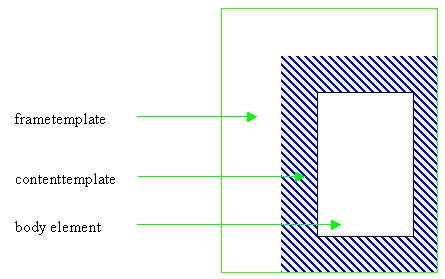
\includegraphics[clip,width=\sgw]{pics/templateMech/frametemplate}
\end{center}
\caption[frametemplate]{frametemplate and contenttemplate}
\label{frametemplatepicture}
\end{figure}


The mastertemplate only defines which frametemplate and which
contenttemplate should be used by the page. We will create a
template set of 

{\dir /system/modules/org.\-opencms.\-default/tem\-plates/template1} (the mastertemplate), 

{\dir /system/modules/org.\-opencms.\-default/frame\-tem\-plates/frametemplate1} 

and {\dir /system/modules/org.\-opencms.\-default/content\-tem\-pla\-tes/con\-tent\-tem\-plate1}. 

To create a template you must first create a new text file in the project's 

{\dir /system/modules/org.\-opencms.\-default/tem\-plates/} 

directory. Go to the 

{\dir /system/modules/org.\-opencms.\-default/tem\-plates/} 

directory in the Explorer view of the new project and start the wizard that creates the new files 
by clicking on the icon with the magic wand.
Select {\name Text} for the type of the file from the New dialog
box (figure~\ref{createOtherType}).

\begin{figure}[hbt]
\begin{center}
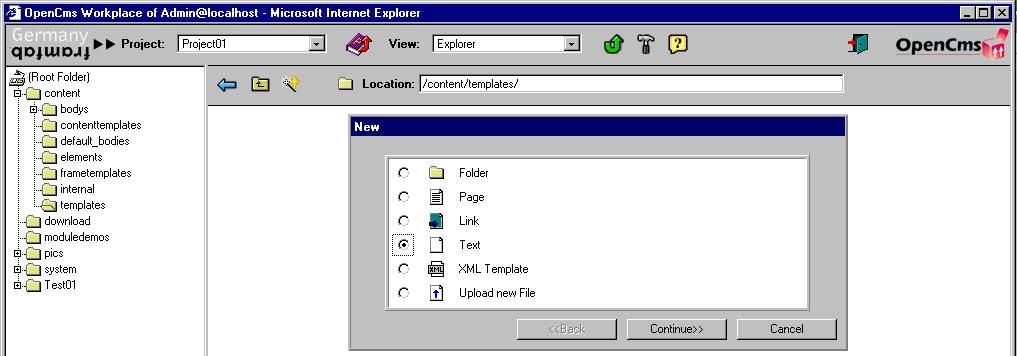
\includegraphics[width=\sgw]
                   {pics/templateMech/createOT}
\caption[Creation of a new template]
           {Select Text for the type of the new file}
\label{createOtherType}
\end{center}
\end{figure}

Enter the name and title for the new template in the Create a new
File dialog box and click on {\name Finish} to end the creation of
the new text file (figure~\ref{createOT2}).

\begin{figure}[hbt]

\begin{minipage}[b]{0.499\linewidth}
  \begin{center}
  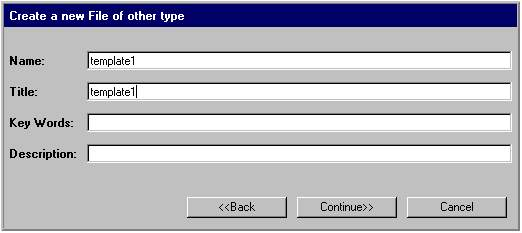
\includegraphics[clip,width=\sgw]
                   {pics/templateMech/createOT2}
 \end{center}
\end{minipage}
\hfill
\caption[Creation of a new template]
           {Enter name and title}
 \label{createOT2}

\end{figure}

\begin{figure}[hbt]
\begin{center}
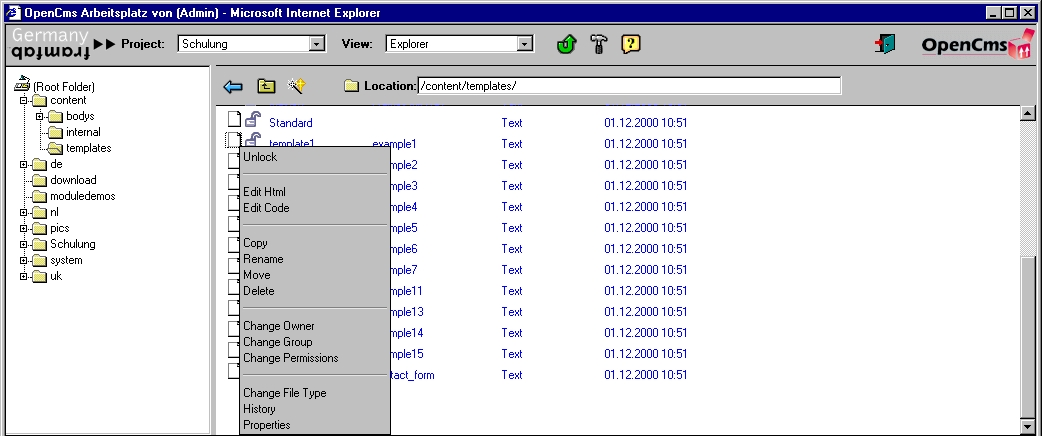
\includegraphics[width=\sgw]
                   {pics/templateMech/editcode}
\caption[select \textit{edit code}]
           {select \textit{edit code} from the context menu}
\label{editcode}
\end{center}
\end{figure}

Select {\name Edit Code} from the file's context menu to edit the
new file. The context menu is accessed by clicking on the new
file's icon (figure~\ref{editcode}). This will start the HTML editor. A
template file is simply an XML file that contains XML and HTML
tags. The mastertemplate contains the definition of the frame-
and the contenttemplate. To accomplish this the template must
contain the following text:

% this should be used to include the examples but it didn't work :-(
%\begin{alltt}
%<?xml version="1.0" encoding="ISO-8859-1"?> 
<XMLTEMPLATE>
    <ELEMENTDEF name="contenttemplate">
        <CLASS>com.opencms.template.CmsXmlTemplate</CLASS>
        <TEMPLATE>/content/contenttemplates/contenttemplate1</TEMPLATE>
    </ELEMENTDEF>
    <ELEMENTDEF name="frametemplate">
        <CLASS>com.opencms.template.CmsXmlTemplate</CLASS>
        <TEMPLATE>/content/frametemplates/frametemplate1</TEMPLATE>
    </ELEMENTDEF>
<TEMPLATE> <ELEMENT name="frametemplate"/> </TEMPLATE>
</XMLTEMPLATE>

%\end{alltt}
\begin{verbatim}
<?xml version="1.0" encoding="ISO-8859-1"?> 
<XMLTEMPLATE>

<ELEMENTDEF name="contenttemplate">
    <CLASS>com.opencms.template.CmsXmlTemplate</CLASS>
    <TEMPLATE>../contenttemplates/contenttemplate1</TEMPLATE>
</ELEMENTDEF> 
<ELEMENTDEF name="frametemplate">
    <CLASS>com.opencms.template.CmsXmlTemplate</CLASS>
    <TEMPLATE>../frametemplates/frametemplate1</TEMPLATE>
</ELEMENTDEF>

<TEMPLATE> 
    <ELEMENT name="frametemplate"/> 
</TEMPLATE>

</XMLTEMPLATE>
\end{verbatim}

You can either type in this text or copy and paste it into the
editor. Exit the editor and save the file by clicking on the icon
to the left that shows a floppy disk and a cross. Now create the
frametemplate1 in the directory 

{\dir /system/modules/org.\-opencms.\-default/frame\-tem\-plates/}

with the text:
%<?xml version="1.0"?> <XMLTEMPLATE>
    <TEMPLATE><![CDATA[
        <html>
            <head>
                <title>The first templates</title>
            </head>
            <BODY >
                ]]><ELEMENT name="contenttemplate"/><![CDATA[
            </BODY>
        </html>]]>
    </TEMPLATE>
</XMLTEMPLATE>

\begin{verbatim}
<?xml version="1.0" encoding="ISO-8859-1"?> 
<XMLTEMPLATE>
    <TEMPLATE><![CDATA[
        <html>
            <head>
                <title>The first templates</title>
            </head>
            <BODY >
                ]]><ELEMENT name="contenttemplate"/><![CDATA[
            </BODY>
        </html>]]>
    </TEMPLATE>
</XMLTEMPLATE>
\end{verbatim}

At last create the contenttemplate1 in 

{\dir/system/modules/org.\-opencms.\-default/content\-tem\-plates/}

with this content:
%<?xml version="1.0" encoding="ISO-8859-1"?> <XMLTEMPLATE>
    <TEMPLATE><![CDATA[
            Hello World! <br>
        ]]><ELEMENT name="body"/>
    </TEMPLATE>
</XMLTEMPLATE>

\begin{verbatim}
<?xml version="1.0" encoding="ISO-8859-1"?> 
<XMLTEMPLATE>
    <TEMPLATE><![CDATA[
            Hello World! <br>
        ]]><ELEMENT name="body"/>
    </TEMPLATE>
</XMLTEMPLATE>
\end{verbatim}

 The next step is to create a new page that uses the template set you just created. As mentioned before,
the page-control file is the one that has to be clicked on to view a page in the Browser.
This file has to be created now. To do so, change to the root folder
and use the wizard to create a new file. Select {\name Page} as the new file type. Enter the web
page's name and title. The name is the name of the file and the title is the title that should
be shown when the page is requested. Select the master template for the new page from the
Template drop-down list, which displays the titles of the templates that can be found in the

{\dir /system/modules/org.\-opencms.\-default/tem\-plates/} 

directory (figure~\ref{chooseMaster}). The other fields in this dialog will be
discussed later. For the time being, they can retain their default values. Click
on the {\name Finish} button to create the new page.

\begin{figure}[hbt]
\begin{center}
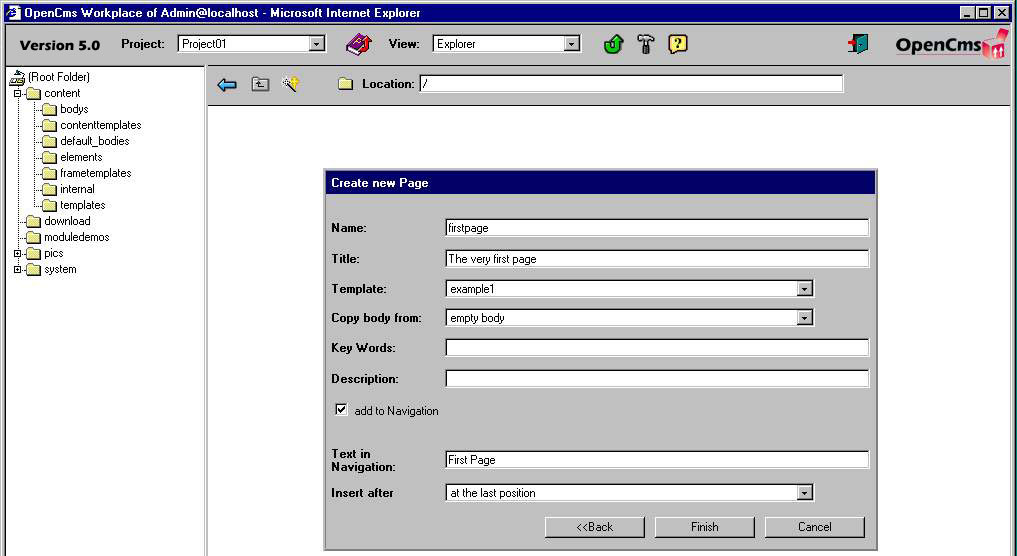
\includegraphics[width=\sgw]
                   {pics/templateMech/chooseMaster}
\caption[choose the master template]
           {The Template drop-down list displays the titles of the templates that are stored in the
            {\dir /system/modules/org.\-opencms.\-default/tem\-plates/} directory}
\label{chooseMaster}
\end{center}
\end{figure}

You can now view the page by clicking on it. A new browser window
will be opened in which the new page is displayed. The page shows
the {\name Hello, world!} text from the contenttemplate. The title
of the page is the title that was defined in the frametemplate.


\subsection{Using methods in XML templates}
%============================================================================

We will now create a new frametemplate that uses a method 
to set the title in the template. This way the title will be set dynamically and
is not the same for all pages created with our template.
To create the new frametemplate you have to create a new
text file (frametemplate2) in the 

{\dir /system/modules/org.\-opencms.\-default/frame\-tem\-plates/}

directory. Follow the steps to create a new template that are
described in the first example, and insert the following text in
your frametemplate:

%<?xml version="1.0" encoding="ISO-8859-1"?> <XMLTEMPLATE>
    <TEMPLATE><![CDATA[
        <html>
            <head>
                <title>]]><method name="getTitle"/><![CDATA[</title>
            </head>
                <BODY >
                    ]]><ELEMENT name="contenttemplate"/><![CDATA[
                </BODY>
        </html>]]>
    </TEMPLATE>
</XMLTEMPLATE>

\begin{verbatim}
<?xml version="1.0" encoding="ISO-8859-1"?> 
<XMLTEMPLATE>
    <TEMPLATE><![CDATA[
        <html>
            <head>
                <title>]]><method name="getTitle"/><![CDATA[</title>
            </head>
                <BODY >
                    ]]><ELEMENT name="contenttemplate"/><![CDATA[
                </BODY>
        </html>]]>
    </TEMPLATE>
</XMLTEMPLATE>
\end{verbatim}
\index{getTitle}

Now you also need a new mastertemplate which uses the new
frametemplate2 and the old contenttemplate.
Create it in 

{\dir /system/modules/org.\-opencms.\-default/tem\-plates/} 

as described in the first example:

%<?xml version="1.0"?> <XMLTEMPLATE>
    <ELEMENTDEF name="contenttemplate">
        <CLASS>com.opencms.template.CmsXmlTemplate</CLASS>
        <TEMPLATE>/content/contenttemplates/contenttemplate1</TEMPLATE>
    </ELEMENTDEF>
    <ELEMENTDEF name="frametemplate">
        <CLASS>com.opencms.template.CmsXmlTemplate</CLASS>
        <TEMPLATE>/content/frametemplates/frametemplate2</TEMPLATE>
    </ELEMENTDEF>
<TEMPLATE> <ELEMENT name="frametemplate"/> </TEMPLATE>
</XMLTEMPLATE>

\begin{verbatim}
<?xml version="1.0" encoding="ISO-8859-1"?> 
<XMLTEMPLATE>
    <ELEMENTDEF name="contenttemplate">
        <CLASS>com.opencms.template.CmsXmlTemplate</CLASS>
        <TEMPLATE>../contenttemplates/contenttemplate1</TEMPLATE>
    </ELEMENTDEF>
    <ELEMENTDEF name="frametemplate">
        <CLASS>com.opencms.template.CmsXmlTemplate</CLASS>
        <TEMPLATE>../frametemplates/frametemplate2</TEMPLATE>
    </ELEMENTDEF>
<TEMPLATE> <ELEMENT name="frametemplate"/> </TEMPLATE>
</XMLTEMPLATE>
\end{verbatim}

You can now create a new page with this mastertemplate and see
that the title of the generated HTML page is exactly the one you typed
in when creating the page. There are a number
of standard methods that can be used when creating
a template. The methods are defined in the 
\textit{com.opencms.template.CmsXmlTemplate} class which is
assigned to the mastertemplate per default in the page-control file.
As you can see, the usage of standard methods is quite simple.

\begin{xml}
  <TITLE>]]><method name="getTitle"/><![CDATA[</TITLE>
\end{xml}

The method-tag is a special tag which allows to call functions from a template. The return
value of the method (in this case the correct title of the page) is inserted into the page when
the template is processed. Other standard methods will be discussed later in this document.

\subsection{The body element}
%============================================================================

To achieve a separation of content and layout of a website, the
content is normally inserted in a body element. A body element is 
a subtemplate, that holds editable content, which will be shown at
the place where this element is located in the contenttemplate. 
Create a new page in the root folder and select the title of the
new template from the drop-down list. For example, if you have
defined the title of the template as template2, this text should
appear in the drop-down list. Enter a title and name for your new
page, and select {\name Finish} to create the page
(figure~\ref{selectTitle}).

\begin{figure}[hbt]
\begin{center}
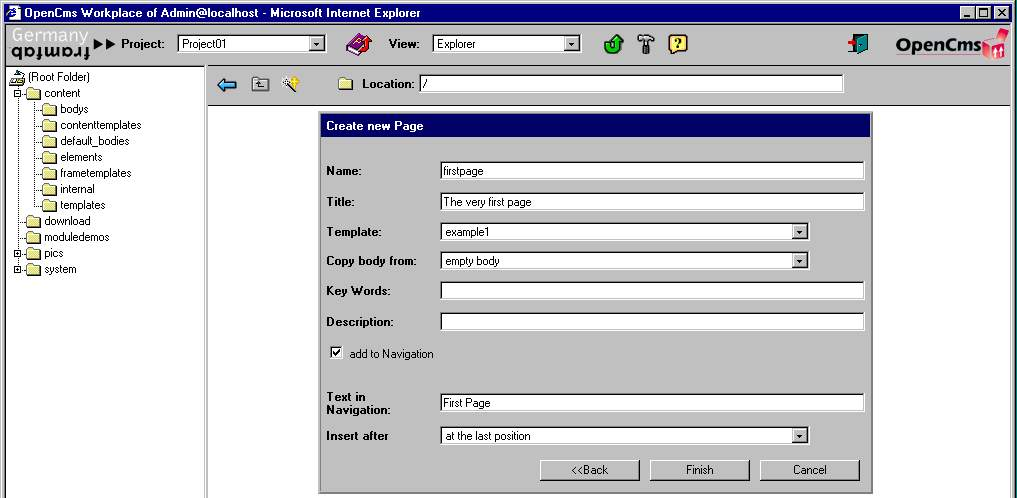
\includegraphics[width=\sgw]
                   {pics/templateMech/setTitle}
\caption[select the title of the template]
           {Select the title of the new template when creating the page}
\label{selectTitle}
\end{center}
\end{figure}

Before we take a look at the new page, we will use the HTML editor
to add text to the body element. To edit the page with the HTML
editor select {\name Edit Page} from the new page's context
menu (figure~\ref{EditPage}).

\begin{figure}[hbt]
\begin{center}
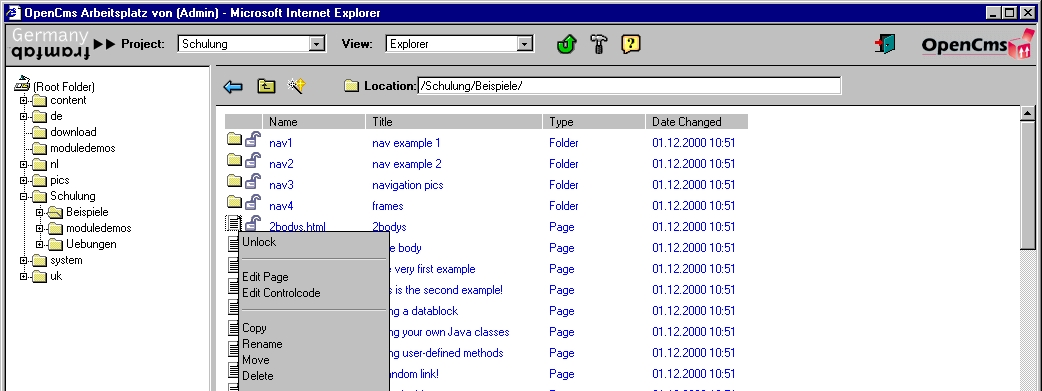
\includegraphics[width=\sgw]
                   {pics/templateMech/editPage}
\caption[{\name Edit Page}]
           {Select {\name Edit Page} from the context menu to edit the page in the HTML editor}
\label{EditPage}
\end{center}
\end{figure}

The editor is a WYSIWYG editor that provides standard HTML file editing functionality. 
You can select the font style and size, insert pictures, and so on.
Entering text in the editor inserts it in the new page's body element (figure~\ref{EditBody}).

\begin{figure}[hbt]
\begin{center}
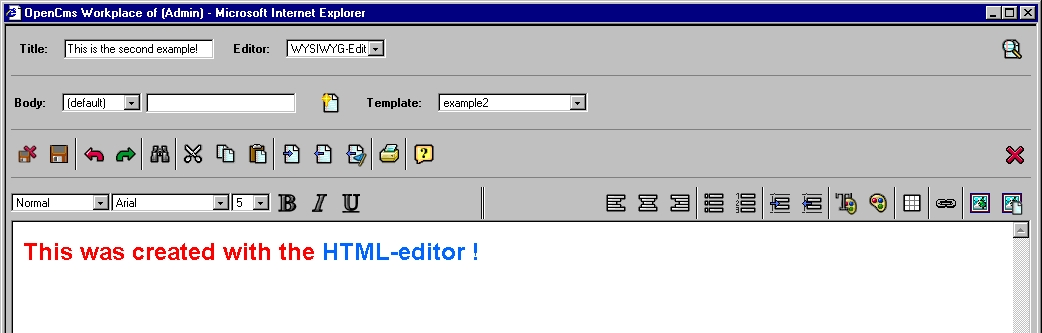
\includegraphics[width=\sgw]
                   {pics/templateMech/HTMLEdit}
\caption[Edit the body]
           {Edit the body with the HTML editor}
\label{EditBody}
\end{center}
\end{figure}

After you have entered your text, close the editor by clicking on the  {\name Save and Exit} icon
to the left. Have a look at the new page by clicking on its name. If you entered the text in
the above example, the page will look like figure~\ref{ThisOutp}.

\begin{figure}[hbt]
\begin{center}
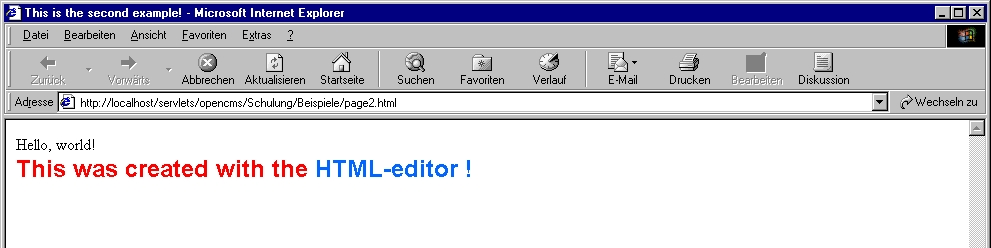
\includegraphics[width=\sgw]
                   {pics/templateMech/ThisOutput}
\caption[The output of the second page]
           {The output of the second page}
\label{ThisOutp}
\end{center}
\end{figure}

As you can see, the first part of the text ({\name Hello, world!})
still comes from the contenttemplate, but the second part, witch
was created with the help of the WYSIWYG editor, comes from the
body element. You can see in the contenttemplate, that the body
template is inserted via the ELEMENT-tag:

\begin{xml}
...\\
\xtaba Hello, world!<br>\\
\xtaba ]]><ELEMENT name="body"/>\\
...\\
\end{xml}

Here, the element with the name {\name body} is inserted after the
{\name Hello, world!} text. The assignment of the element  {\name
body} to the body template in the {\dir /system/bodies/} directory
is made in the page-control file.
\clearpage


\subsection{Defining the layout in the frametemplate}
%============================================================================

We will now go a little step further and come closer to the recommended layout of a XML template generated
website. Normally, a website is more or less designed like in figure~\ref{MasterAndElems}.

\begin{figure}[hbt]
\begin{center}
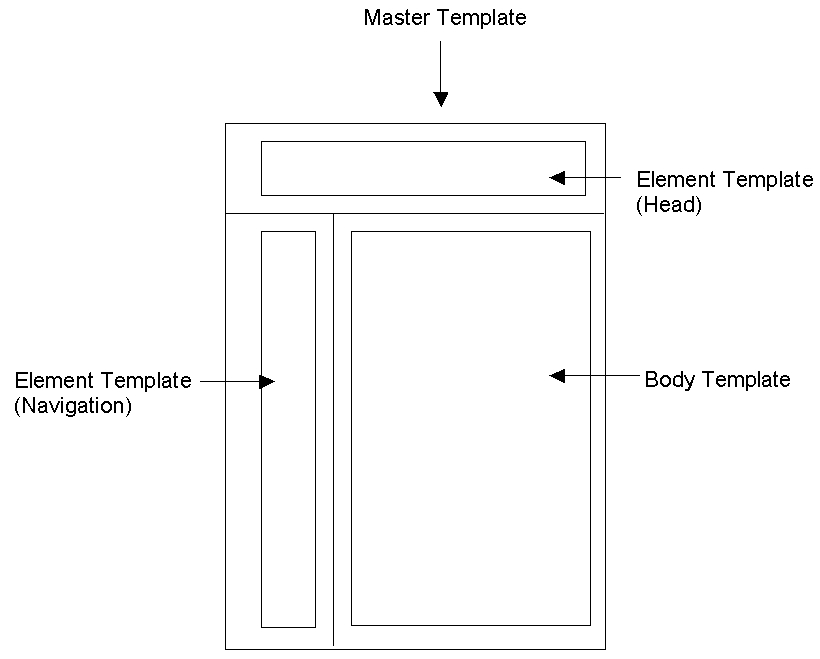
\includegraphics[width=\sgw]
                   {pics/templateMech/MasterAndElementes}
\caption[Master and Elementes]
           {Frametemplate and Elements}
\label{MasterAndElems}
\end{center}
\end{figure}

A head-section for logos and things like that, an element for the
navigation and a content area for the content. This layout can for
example be realized with a table defined in the frametemplate and
three elements which are inserted. To  create a page with this
layout, you should first create the frametemplate3 with the table
in the 

{\dir /system/modules/org.opencms.default/frametemplates/} 

directory.  The creation can be done similar to the way we did it before. You can then add the
following code to the frametemplate3:
%<XMLTEMPLATE>
<TEMPLATE><![CDATA[
    <HTML>
        <HEAD>
            <TITLE>]]><method name="getTitle"/><![CDATA[</TITLE>
        </HEAD>
        <BODY>
            <TABLE border width="100%" height="100%">
                <TR height="30%">
                    <TH colspan=2 width="100%" align="center">
                        The Head section
                    </TH>
                </TR>
                <TR height="70%">
                    <TD width="20%" align="center" valign="top">
                        Navigation
                    </TD>
                    <TD width="80%" align="center">
                        ]]><ELEMENT name="contenttemplate"/><![CDATA[
                    </TD>
                </TR>
            </TABLE>
        </BODY>
    </HTML>]]>
</TEMPLATE>
</XMLTEMPLATE>

\begin{verbatim}
<XMLTEMPLATE>
<TEMPLATE><![CDATA[
    <HTML>
        <HEAD>
            <TITLE>]]><method name="getTitle"/><![CDATA[</TITLE>
        </HEAD>
        <BODY>
            <TABLE border width="100%" height="100%">
                <TR height="30%">
                    <TH colspan=2 width="100%" align="center">
                        The Head section
                    </TH>
                </TR>
                <TR height="70%">
                    <TD width="20%" align="center" valign="top">
                        Navigation
                    </TD>
                    <TD width="80%" align="center">
                        ]]><ELEMENT name="contenttemplate"/><![CDATA[
                    </TD>
                </TR>
            </TABLE>
        </BODY>
    </HTML>]]>
</TEMPLATE>
</XMLTEMPLATE>
\end{verbatim}

You also need a new mastertemplate in 

{\dir /system/modules/org.\-opencms.\-default/tem\-plates/}

where you use the new frame\-template and an empty contenttemplate:
%<?xml version="1.0" encoding="ISO-8859-1"?> 
<XMLTEMPLATE>
    <ELEMENTDEF name="contenttemplate">
        <CLASS>com.opencms.template.CmsXmlTemplate</CLASS>
        <TEMPLATE>/content/contenttemplates/empty</TEMPLATE>
    </ELEMENTDEF>
    <ELEMENTDEF name="frametemplate">
        <CLASS>com.opencms.template.CmsXmlTemplate</CLASS>
        <TEMPLATE>/content/frametemplates/frametemplate3</TEMPLATE>
    </ELEMENTDEF>
<TEMPLATE> <ELEMENT name="frametemplate"/> </TEMPLATE>
</XMLTEMPLATE>

\begin{verbatim}
<?xml version="1.0" encoding="ISO-8859-1"?> 
<XMLTEMPLATE>
    <ELEMENTDEF name="contenttemplate">
        <CLASS>com.opencms.template.CmsXmlTemplate</CLASS>
        <TEMPLATE>../contenttemplates/empty</TEMPLATE>
    </ELEMENTDEF>
    <ELEMENTDEF name="frametemplate">
        <CLASS>com.opencms.template.CmsXmlTemplate</CLASS>
        <TEMPLATE>../frametemplates/frametemplate3</TEMPLATE>
    </ELEMENTDEF>
<TEMPLATE> <ELEMENT name="frametemplate"/> </TEMPLATE>
</XMLTEMPLATE>
\end{verbatim}


As you can see, the text for the head-section and the
navigation-section is just inserted dircetly in the frametemplate,
but the content is inserted as an element. The empty
contenttemplate just inserts the body element. Please create a new
page which uses the new mastertemplate with the wizard and edit
the body with the WYSIWYG editor so that you can see some output.
Afterwards the output could look like in figure~\ref{MasterEl}.

\begin{figure}[hbt]
\begin{center}
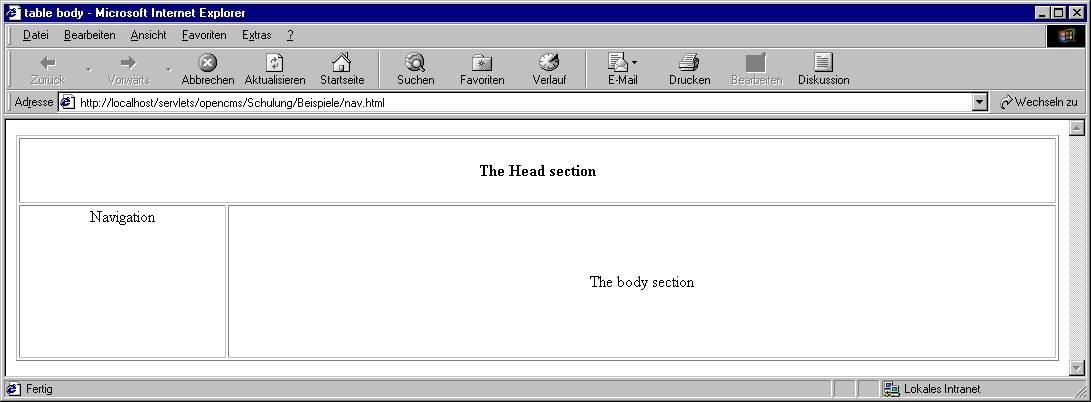
\includegraphics[width=\sgw]
                   {pics/templateMech/simpleTable}
\caption[Master and subelementes]
           {Master and subelementes}
\label{MasterEl}
\end{center}
\end{figure}

This example should give a little insight in how to handle
standard HTML features as e.g. tables and the XML tags together.
You can now try to change the layout of the page and edit the
frametemplate and contenttemplate. 

\section{XML templates and directories}
%============================================================================

\subsection{The XML structure of a template}
%============================================================================

\index{XML}
XML is a markup language, which is just like HTML defined by SGML and is used to store content
in a structured way.  The main difference,is that one is able to 
define his own tags. By that, it is possible to achieve
a separation between content and layout.
While HTML allows to define how something should be displayed XML allows to define items that
belong logically together.
For example, it is possible to define blocks of surnames, adresses etc..
XML is a powerfull markup language, but you don�t need to know much about it for understanding
the XML template mechanism.
The XML template mechanism uses XML to deposit HTML fragments single and structured. 
These fragments can then be fetched
specifically and used dynamically.
From the technical side of view, there is no difference between the master and the body (sub)
templates. Both are XML-files with the same syntax. The difference is more a logical one. The
following section explains the structure of a template file.
Below is the general framework of a template file:
\index{XML-tags}
\begin{xml}
<?xml version="1.0" encoding="ISO-8859-1"?>\\
<XMLTEMPLATE>\\
<!-- user-defined data blocks or elementdefintions -->\\
<TEMPLATE>\\
\xtaba <![CDATA[\\
\xtaba   <!-- HTML-code -->\\
\xtaba   ]]> <XML-TAGS> [![CDATA[\\
\xtaba   <!-- the  HTML-code  continues here... -->\\
\xtaba
\xtaba      ]]>\\
</TEMPLATE>\\
<!-- user-defined data blocks or elementdefinitions -->\\
</XMLTEMPLATE>\\
\end{xml}
\index{XMLTEMPLATE}
\index{TEMPLATE}

The first line determines the type of the document and must be placed at the very beginning of
the document. Leading spaces are not allowed. The whole template is enclosed between
{\tag <XMLTEMPLATE>} tags. Inside this tag the template is defined between the start
{\tag <TEMPLATE>} tag and
the end {\tag </TEMPLATE>} tag. HTML code can be placed in the template between the CDATA tags,
which starts with
{\tag <![CDATA[ } and ends with {\tag ]]>}.
Everything between CDATA tags is ignored by the XML
parser and directly streamed to the output. XML tags that are used in the template must be
placed outside of the {\tag CDATA} tags.  Examples for XML tags that can be used have been shown
in the first examples. You will primarily place process, element, or method tags in your document.
Outside the template tags and inside the {\name xmltemplate} tags you can place data blocks
or element definitions.
\index{CDATA}

\subsection{Directory structure}

The templates, body templates and element templates etc. are 
stored in different standard directories of the VFS. 
If you create a new file of the type {\name Page}
within a project, a page-control file is created in the
current directory. Also a body-template is created with the same name as the page
in the {\dir /system/bodies/} directory under the same directory structure.
For example if you create a page in the folder /examples the body-template will be located
in /system/bodies/examples. 
If you click on the page-control file and choose {\name Edit Page} 
from the context menu, you actually edit the body in the 
{\dir /system/bodies/} directory with
the WYSIWYG editor. You can check this out by looking at both
files with the source-code editor after you have changed
something, but you should never change the files in the body directory
directly.

\subsection{The subdirectories of the content folder}
\index{content}

\subsubsection{- templates:} \index{templates}

In the directory 

{\dir /system/modules/org.\-opencms.\-default/tem\-plates/} 

are the definitions for the different combinations of frame- and contenttemplates. These
files have always the same structure as you have seen in the
examples so far. The only things that can be changed are the names
of the two templates (only names not the path!). Never add any
other html or xml stuff here.

\subsubsection{- frametemplates:} \index{frametemplates}

In the frametemplates the design of the page is build. e.g. it
can contain the navigation and an head element. There is always
the area where the contenttemplate is included which was defined
in the mastertemplate.

\subsubsection{- contenttemplates:} \index{contenttemplates}

The contenttemplates defines the content part of the page. It includes the body element
and maybe other elements.

\subsubsection{- bodys:} \index{bodys}

This folder is for internal use only. It contains the above
mentioned body elements.

\subsubsection{- default\_bodies:} \index{defaultbodies}

In this folder you can store some bodies which you use often. When
you create a new page you can choose one of these bodies to be
copied in your new pagebody.

\subsubsection{- internal:} \index{internal}

This directory is not used any more. It is still there for
compatibility reasons and its job is now taken over by the
elements folder.

\subsubsection{- elements:} \index{elements}

Here you can store your dynamic elements. An element is dynamic if
it doesn't use the standard class CmsXmlTemplate. For Example the
navigation element.

\clearpage 


\section{Details of the proprietary XML template mechanism}
%============================================================================

\subsection{Using data blocks}
\label{using datablocks}
Up to here, you got an overview over the template mechanism, but many things which have already
been used have not been explained. We will now go one step back and take a look at some earlier
examples and the basic structures of the template mechanism.

In this example you will learn how to use data blocks in a
template. A data block is a named block of text that can contain
XML and HTML code. We will change the earlier example by putting
the {\name Hello, world!} text into a data block with the name
{\name message.} To create the new contenttemplate, create a new
text file named contenttemplate2 in the 

{\dir /system/modules/org.\-opencms.\-default/content\-tem\-plates/} 

directory with the following text:
\index{data blocks}

%<?xml version="1.0"?>
<XMLTEMPLATE>
    <MESSAGE><![CDATA[Hello world!]]></MESSAGE>
    <TEMPLATE><![CDATA[
            ]]><PROCESS>message</PROCESS><![CDATA[ <br>
        ]]><ELEMENT name="body"/>
    </TEMPLATE>
</XMLTEMPLATE>

\begin{verbatim}
<?xml version="1.0" encoding="ISO-8859-1"?>
<XMLTEMPLATE>
    <MESSAGE><![CDATA[Hello world!]]></MESSAGE>
    <TEMPLATE><![CDATA[
            ]]><PROCESS>message</PROCESS><![CDATA[ <br>
        ]]><ELEMENT name="body"/>
    </TEMPLATE>
</XMLTEMPLATE>
\end{verbatim}

Note the changes that have been made in the template. The {\name Hello, world!} text is now
enclosed between {\tag <MESSAGE>} and {\tag </MESSAGE>}, which are the start and end tags for
the data block. You can
select an arbitrary name for the data block, which must be defined outside the template tag and
inside the xmltemplate tag. In the body section of the HTML code there is now a
{\tag <PROCESS>} tag
with the text {\name message} enclosed in it. This process tag will insert the data block with the
name {\name message} in the document. The output of this example is exactly the same as the one of the
first example, assuming you haven't added text to the body in the HTML editor.

\begin{figure}[hbt]
\begin{center}
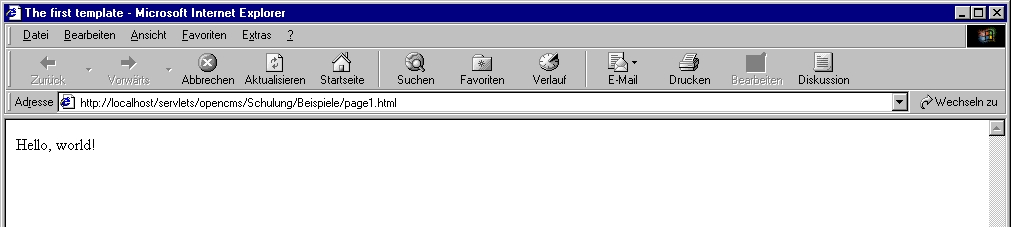
\includegraphics[width=\sgw]
                   {pics/templateMech/OutputHelloWorld}
\caption[The output of this example]
           {The output of this example}
\label{output}
\end{center}
\end{figure}

You can of course edit the body if you want to insert additional
text or pictures in the document. Data blocks can be used to
insert blocks of XML or HTML code in your document. The content of
these blocks can also be defined dynamically in Java classes. The
next example will show how to do this.

\subsection{Setting data blocks dynamically}
\label{setting data blocks dynmically}
We do already now how data blocks are used in templates.
In this example we will define the content of the data block in a Java
method. That means we will write our own class that controls the output
of the template and places the text in the data block. To place
something in a data block that can dynamically be changed we will use
the {\tag <PROCESS>} tag inside of the data block. This functionality will be
enclosed in an element which we will place inside the contenttemplate. Note that
functionality which requires Java programming should always be placed inside an element
and not the frametemplate or contenttemplate itself, because these two templates are always
associated with the default {\class org.opencms.file.CmsXmlTemplate} class and not a
userdefined class. Here is the text that the contenttemplate should contain:

\begin{verbatim}
<?xml version=1.0 encoding="ISO-8859-1"?>
<XMLTEMPLATE>
<TEMPLATE>
    <ELEMENT name="example4"/>
    <ELEMENT name="body"/>
</TEMPLATE>
<ELEMENTDEF name="example4">
    <CLASS>CmsExample4</CLASS>
    <TEMPLATE>../elements/example4</TEMPLATE>
</ELEMENTDEF>
</XMLTEMPLATE>
\end{verbatim}

As you can see we have included an additional element example4 inside the contenttemplate
with the name example4. Inside the {\tag <ELEMENTDEF>} tag we define which Java class and template
is used to create the output of this element.
Create a file contenttemplate4 with the above content and make a new mastertemplate
which uses this contenttemplate. The next step is to create the element template.
Create a new text file example4 in the folder 

{\dir /system/modules/org.opencms.default/elements/}

with the following content:

\begin{verbatim}
<?xml version= "1.0" encoding="ISO-8859-1"?>
<XMLTEMPLATE>

<MESSAGE>
    <![CDATA[Hello, World ]]>
    <PROCESS>greeting</PROCESS>
</MESSAGE>

<TEMPLATE>
   <PROCESS>message</PROCESS>
</TEMPLATE>

</XMLTEMPLATE>
\end{verbatim}

The template contains a data block {\tag <MESSAGE>} with  a {\tag <PROCESS>} tag inside it.
The {\tag <PROCESS>} tag is used to place the processed input of data blocks in a template.
The  text {\tag <PROCESS>greeting</PROCESS>} in the template will be replaced by the processed
value of the data block with the name greeting. The content of this data block is not defined yet, it
will be defined dynamically inside the Java class.
Next create a new page and select the newly created mastertemplate as the template for this page.
The next step is to write the Java class that controls the output of
our new template. The new class will be derived from the {\class com.opencms.template.CmsXmlTemplate}
class. This class provides the basic functionality and methods to control template
files. In the new class we will override the {\meth getContent()} method. This
method creates the output of the template and is invoked
automatically by the system. 

This is the source code for our new class:

\begin{java}
import com.opencms.template.*;\\
import org.opencms.file.*;\\
import org.opencms.main.*;\\

import java.util.*;\\

public class CmsExample4 extends CmsXmlTemplate \{\\
\index{getContent}
\jtaba public byte[] getContent(CmsObject cms,\\
\jtabc        String templateFile, String elementName,\\
\jtabc        Hashtable parameters,String templateSelector)\\
\jtabc        throws CmsException \{\\
\jtabb        CmsXmlTemplateFile templateDocument =\\
\jtabb        getOwnTemplateFile(cms, templateFile, elementName, parameters,\\
\jtabd                           templateSelector);\\

\jtabb        templateDocument.setData("greeting","from Java!");\\
\jtabb        return startProcessing(cms, templateDocument, \\
\jtabd                               elementName, parameters, templateFile);\\
\jtaba    \}\\
\}\\
\end{java}

The first method we use is {\meth getOwnTemplateFile()}. This method parses the 
XML template and creates an object of {\class com.opencms.template.CmsXmlTemplateFile}
which contains the templatefile as a DOM-object and has methods to manipulate the data blocks
of the template. This method call is a standard call that will always be used inside the
{\meth getContent()} method to access the template file. The next method we use
is the setData() method. This method sets a data block in the template with a given String
value. The first parameter of method {\meth getData()} takes the name of the data block and the second its
value. As you can see we fill a data block named greeting with the value "from Java". This means that
now if this data block is used in the template it will have the value "from Java". The final method call
in the method {\meth getContent()} invokes the method {\meth startProcessing()} which results in the 
processing and generating of the output of the whole template. 
The return value of this method is the ouput of the template and will
be returned by the {\meth getContent()} method. The calls to method {\meth getOwnTemplateFile()} 
and {\meth startProcessing()} are used in almost every case when writing a {\meth getContent()} 
method because they provide a rather basic functionality that allows manipulating and processing of the template.

You can compile the class and place the generated {\class Example4.class} file
in the subdirectory {\dir WEB-INF/classes/} of your webapp. 
To load the new class you have to restart the webapplication. If everything
works fine you should see something like in figure~\ref{OutputJavaClass}.

\begin{figure}
\begin{center}
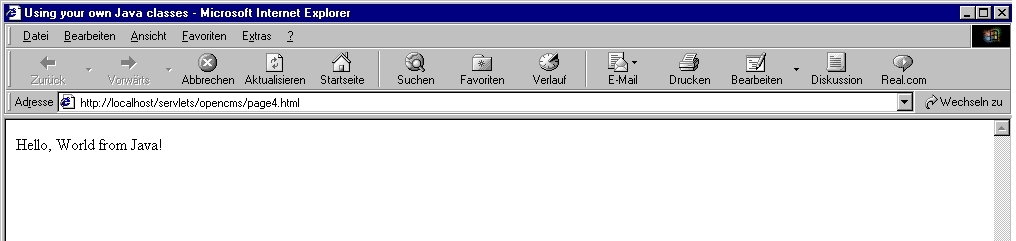
\includegraphics[clip,width=\sgw]{pics/modules/30}
\end{center}
\caption[Output generated using the new Java class]{Output generated using the new Java class}
\label{OutputJavaClass}
\end{figure}

\subsection{Using user-defined methods}
\label{userdefined methods}
In the last example we saw one way of creating dynamic content in a
template. Another way is to use user-defined methods in the template.
You have already seen how to use the {\meth getTitle(}) method in a template in
the second example. If you want to write your own methods, you can
derive a class from the existing template class
{\class com.opencms.template.Cms\-Xml\-Template} and add your own methods.

We will write a method that returns the string {\name Hello, World from Java!} and give it the
name {\meth getHello(}). The return value of the method will be placed inside the template where
we call the method with the {\tag <METHOD>} tag. You should create another contenttemplate which includes an element example5
and a new mastertemplate which uses this contenttemplate. You have to create a new element template {\name example5}, or if 
you want to use the contenttemplate and mastertemplate of the previous example 
you can also just replace the element of the previous example with the following content:

\begin{verbatim}
<?xml version="1.0" encoding="ISO-8859-1"?>
<XMLTEMPLATE>
<TEMPLATE>
    <METHOD name="getHello"/>
</TEMPLATE>
</XMLTEMPLATE>
\end{verbatim}

A new Java class {\class CmsExample5} defines the method {\meth getHello(}):

\begin{java}
import com.opencms.template.*;\\
import org.opencms.file.*;\\
import org.opencms.main.*;\\

import java.util.*;\\

public class  CmsExample5 extends  CmsXmlTemplate \{\\

\xtabb   public Object getHello(CmsObject cms, String tagcontent,\\
\xtabe           A\_CmsXmlContent doc, Object userObject) \{\\
\xtabc       return "Hello, World from Java!";\\
\xtabb   \}\\

\}\\
\end{java}

Note that the signature of user-defined methods is always the same and cannot be changed.
To use the class, compile it and place it in the subdirectory {\dir WEB-INF/classes/} of your
webapp. Create a new page that uses the new mastertemplate. 

The output of the new template will be the same as that of the previous
example: it displays the string {\name Hello, World from Java!} on the screen.
The only difference is the procedure we followed to accomplished the
task of inserting something in the document. In the previous example we
set a datablock with the {\meth setData()} method and now we used the
a new user-defined method {\meth getHello()}.

\subsection{The relationship between templates, page-control files, and
Java classes}

For every new page that is created with an XML template the system
automatically creates a {\name page-control} file. This page-control file
determines the mastertemplate that is used by the new page and contains
the element definition of the body element. Examples for page-control files
have already been shown before. 
Below is the page-control file for an earlier example:

\begin{xml}
<?xml version= "1.0" encoding="ISO-8859-1"?>\\
<page>\\
\xtaba <CLASS>com.opencms.template.CmsXmlTemplate</CLASS>\\
\xtaba <MASTERTEMPLATE>/system/modules/org.\-opencms.\-default/tem\-plates/template5</MASTERTEMPLATE>\\
\xtaba <ELEMENTDEF name="body">\\
\xtaba <CLASS>com.opencms.template.CmsXmlTemplate</CLASS>\\
\xtaba <TEMPLATE>/system/bodies/page5.html</TEMPLATE>\\
\xtaba </ELEMENTDEF>\\
</page>\\
\end{xml}

The name of the mastertemplate file is enclosed
between the {\tag <MASTERTEMPLATE>} tags. The {\tag <CLASS>} tag above it determines the
Java class that controls the mastertemplate. This class is the  generic
{\class com.opencms.template.CmsXmlTemplate} class and is  always used to
control the mastertemplate. The {\tag <ELEMENTDEF>} tag defines the class and template 
used for the body element. The body element is the one that contains
the HTML-code generated with the WYSIWYG editor. 
An element definition must be provided for every subelement. 
The body element can be placed inside a template with the element tag as
follows:

{\tag <ELEMENT name="body"/>}

You can place other subtemplates in your document in the same way you
placed the body template in it, by inserting a
{\tag <ELEMENT name="aName"/>} tag and element definition in your document.
The name for the new element can be freely defined.
The controlling Java class for the body template is always the class
{\class com.opencms.template.CmsXmlTemplate} because a body element does
not have any user-defined functionality.


\subsection{Process, Method and Element Tags}
%============================================================================

The {\name process}, {\name method} and {\name element} tags enable you to insert dynamic
content in your template. They have already been used in the first
examples. Their syntax and details of their usage will be discussed in the
following sections.


\subsubsection{The Process Tag}
%============================================================================

The {\name process} tag can be used to insert the content of data blocks in
your document. The data blocks can be defined in the document or set by
Java classes. We will explain how a process tag works by taking a look
at the example of section \ref{using datablocks} on page \pageref{using datablocks}.
Here is the content of the contenttemplate for this example:

\begin{verbatim}
<?xml version= "1.0" encoding="ISO-8859-1"?>
<XMLTEMPLATE>
<MESSAGE>
    <![CDATA[Hello, World ]]>
    <PROCESS>greeting</PROCESS>
</MESSAGE>

<TEMPLATE>
    <PROCESS>message</PROCESS>
</TEMPLATE>
</XMLTEMPLATE>
\end{verbatim}

There are two process tags in this template: the first inside the data
block {\name message} and the second inside the template tag. The text inside
the process tag defines the data block that will be processed. In this
example two data blocks will be processed, one named {\name greeting} and one
named {\name message}. The {\name message} data block is defined in the template
document. The data block {\name greeting} is not defined in the document, but
set in the Java class that is associated with the template. The
{\meth setData()} method was used to accomplish this:

{\meth templateDocument.setData("greeting","from Java!");}

Calling the method {\meth setData} here has the same effect as adding a datablock
of the form:
\begin{xml}
<greeting><![CDATA[from Java!]]></greeting>
\end{xml}
into the template. The difference is that it is set dynamically by a Java method
and not statically inside the template. 

\label{random link example}
To show that it is possible to set the data block dynamically to different values
inside a Java class, the next example inserts a randomly selected link into a template.
The Java program randomly selects one of two data block values for a link's target attribute.

Create a new contenttemplate which includes a new element with the following content:

\begin{xml}
<?xml version="1.0" encoding="ISO-8859-1"?>\\
<XMLTEMPLATE>\\
<LINK1>www.opencms.org</LINK1>\\
<LINK2>www.yahoo.de</LINK2>\\
<TEMPLATE>\\
<![CDATA[\\
<a href="http://]]><PROCESS>link</PROCESS><![CDATA[">\\
Where will we go?</a>\\
]]>\\
</TEMPLATE>\\
</XMLTEMPLATE>\\
\end{xml}

The template defines a hypertext link where the value of the target attribute
is defined by a data block named {\name link}.
The value of the data block is set inside the template with the {\tag <PROCESS>} tag.
The value of the data block {\name link} will be set randomly in a Java class.
This is the source code for the new class:

\begin{java}
import com.opencms.template.*;\\
import org.opencms.file.*;\\
import org.opencms.main.*;\\

import java.util.*;\\[1ex]

public class CmsExample6 extends CmsXmlTemplate \{\\[1ex]

\jtaba public byte[] getContent(CmsObject cms,\\
\jtabc        String templateFile, String elementName,\\
\jtabc        Hashtable parameters,String templateSelector)\\
\jtabc        throws CmsException \{\\
\jtabb   String linkTarget;\\
\jtabb   linkTarget = "LINK"\\
\jtabd       + String.valueOf((int)(Math.random()*2+1));\\
\jtabb   CmsXmlTemplateFile templateDocument =\\
\jtabd       getOwnTemplateFile(cms, templateFile, elementName,\\
\jtabd       parameters,templateSelector);\\
\jtabb   templateDocument.setData("link",\\
\jtabd       templateDocument.getDataValue(linkTarget));\\
\jtabb   return startProcessing(cms, templateDocument, elementName,\\
\jtabd       parameters, templateFile);\\
\jtaba \}\\[1ex]

\jtaba public CmsCacheDirectives getCacheDirectives(CmsObject cms,\\
\jtabd     String templateFile, String elementName,\\
\jtabd   Hashtable parameters, String templateSelector) \{\\
\jtabb   return new CmsCacheDirectives(false);\\
\jtaba \}\\
\}\\
\end{java}
\index{getCacheDirectives()}
\index{CmsCacheDirectives}

The data block that is used for the link's target is randomly selected in
the line:

\begin{java}
linkTarget = "LINK"\\
\jtabd              + String.valueOf((int)(Math.random()*2+1));\\
\end{java}

This statement produces a string {\name "Link1"} or {\name "Link2"} based on the number
that is randomly created by the expression {\name (Math.random()*2+1)}.
The value of the data block link is defined in the following expression:

{\code templateDocument.setData("link",\\
  templateDocument.getDataValue(linkTarget));}

The data block named {\name link} is defined with the method {\meth setData()} and
the content of the data block is the value of the data block that will
be fetched with {\meth getDataValue(linkTarget)}. Because the variable
{\name linkTarget} has either the value {\name "Link1"} or {\name "Link2"} the link will be
defined with the content of data block {\name "Link1"} or{\name  "Link2"}.
To ensure that the link is refreshed every time the page is requested,
the class overrides the method {\meth getCacheDirectives()}. This method controls
the way XMl template elements are cached. The implementation in the superclass
{\class com.opencms.template.CmsXmlTemplate} uses the caching mechanism and would prevent the element
from being refreshed every time it is requested. The details of the element caching mechanism 
are explained in section \ref{element cache}(page \pageref{element cache}).
At this point it is only necessary to know that if an element should be dynamically created
on every request the method {\meth getCacheDirectives()} has to be implemented in the template class
in the way we did in this example.

\label{animal list example}
The next example will show how to create tables or lists using the
{\tag process} tag. You can use the {\tag process} tag to set the data entries in
tables in Java classes. The table will be dynamically built in the Java
class by producing a string by concatenating table rows. The
layout of the table is defined inside the template. The element template could
look like this:

\begin{xml}
<?xml version="1.0" encoding="ISO-8859-1"?>\\
<XMLTEMPLATE>\\

<TEMPLATE>\\
<![CDATA[ <H1>Animal list</H1>\\
<table border=1>\\
]]>\\
\xtaba <process>tablehead</process>\\
\xtaba <process>list</process>\\
<![CDATA[\\
</table>\\
]]>\\
</TEMPLATE>\\
<tablehead>\\
<![CDATA[\\
\xtaba <tr>\\
\xtabb <td>Nr</td>\\
\xtabb <td>animal</td>\\
\xtabb <td>owner</td>\\
\xtaba </tr>\\
]]>\\
</tablehead>\\
<row>\\
<![CDATA[\\
\xtaba <tr>\\
\xtabb <td>]]><process>number</process><![CDATA[</td>\\
\xtabb <td>]]><process>name</process><![CDATA[</td>\\
\xtabb<td> ]]><process>owner</process><![CDATA[</td>\\
\xtaba </tr>\\
]]>\\
</row>\\
</XMLTEMPLATE>\\
\end{xml}


The template defines a table and two data blocks. The data block
{\tag tablehead} defines a static heading for every column and will be
inserted in the table by the {\tag process} tag. The table content will
be created by a Java class and will be set as the data block {\name list.}
The layout of the table's rows is defined by the data block {\name row.} The Java
class will set the value for {\name number}, {\name name} and {\name owner}
for every row and concatenate the values of the resulting rows and
insert them in the document as the data block {\name list.} Here is the
source code of the Java class:

\begin{java}
import org.opencms.file.*;\\
import com.opencms.template.*;\\

import java.util.*;\\[1ex]

public class CmsExample7 extends CmsXmlTemplate \{\\

public byte[] getContent(CmsObject cms, String templateFile,\\
\jtabc        String elementName, Hashtable parameters,\\
\jtabc        String templateSelector) throws CmsException \{\\
\jtabb    String[] owners =\\
\jtabc       {"Martin","Thomas","Andreas","Bill","Michael","Doris"};\\
\jtabb    String[] animals =\\
\jtabc       {"cat","dog","mouse","rat","bird","snake"};\\
\jtabb    CmsXmlTemplateFile template =\\
\jtabd        getOwnTemplateFile(cms,templateFile,elementName,\\
\jtabd        parameters,templateSelector);\\
\jtabb    String list = "";\\
\jtabb    for (int i=0; i < animals.length;  i++) \{\\
\jtabd        template.setData("number", i+"");\\
\jtabd        template.setData("name",animals[i]);\\
\jtabd        template.setData("owner",owners[i]);\\
\jtabd        String row = template.getProcessedDataValue("row");\\
\jtabe           list += row;\\
\jtabb    \}\\
\jtabb    template.setData("list",list);\\
\jtabb    return startProcessing(cms, template, elementName,\\
\jtabd        parameters, templateSelector);\\
\jtabb    \}\\
\}\\
\end{java}
\index{CmsXmlTemplateFile}
\index{getOwnTemplateFile}
The Java class overrides the method {\meth getContent()} that creates the
template's output. Two string arrays are defined in this method that
hold the entries for the owners and the animals that will be inserted
in the table. The rows are generated by setting the data blocks
{\name number}, {\name name} and {\name owner} and fetching the
processed data block {\name row} (this means the process tags have been
replaced by the corresponding values of the data blocks). The result is concatenated
in a string and set as the data block {\name list.} The final call to
{\meth startProcessing()} starts the generation of the template's output.
The last example can be modified to produce a list instead of a table.
The Java class can be left unchanged and reused to create the list.
This shows that it is possible to change the layout in the template
without having to change the Java class. This is the template that will
generate a list instead of a table:

\begin{xml}
<?xml version="1.0" encoding="ISO-8859-1"?>\\
<XMLTEMPLATE>\\

<TEMPLATE>\\
<![CDATA[ <H1>Animal list 2</H1>\\
<ul>\\
\xtabb    ]]>\\
\xtabb    <process>list</process>\\
\xtabb    <![CDATA[\\
</ul>\\
]]>\\
</TEMPLATE>\\
<row>\\
<![CDATA[\\
\xtaba <li>\\
\xtabb ]]><process>name</process><![CDATA[,\\
\xtabb ]]><process>owner</process><![CDATA[\\
\xtaba </li>\\
]]>\\
</row>\\
</XMLTEMPLATE>\\
\end{xml}

The template places the data block {\name list} in an unordered list. The
row's layout has been changed to list entries. The name and the owner
are set in the Java class and the list is generated in the same way
that it was in the last example. Note that the data block number is not
used by the template, but still set in the Java class. Although this is
unneeded, it is harmless because the data block is set without being
processed.

\subsubsection{The Method Tag}
%============================================================================

The method tag is used to insert the output of a method in a document.
You can define your own method inside a class derived from {\class com.opencms.template.CmsXmlTemplate}
or use the standard methods in this class. In section \ref{userdefined methods} (page \pageref{userdefined methods}) 
we created the new method {\meth getHello()} to show how method tags are used.
In general, a method is used in a template by inserting a {\tag <METHOD>} tag.
A method can take parameters that are passed to the method by
specifying them in the method tag.

The syntax for the method tag:

{\meth - <method name="test"/>

- <method name="test2">parameter(s)</method>}

The name attribute of the {\tag <METHOD>} tag specifies the method to call
and is case sensitive. A parameter can be passed to the method as a string
value enclosed by the {\name method} tag. For methods that don't need any
parameters, the end tag {\tag </METHOD>} can be omitted and the tag can be
closed by entering {\tag />}. When parameters are passed as a string to a
method, the method tag has to be closed with the
corresponding end tag {\tag (</METHOD>)}.The previous examples that generated a table
and a list using a process tag can easily be modified to use a method
instead. The next example will show how to generate a table with a
new method {\meth getTable()}. Here is the element template:

\begin{xml}
<?xml version="1.0" encoding="ISO-8859-1"?>\\
<XMLTEMPLATE>\\

<TEMPLATE>
<![CDATA[ <H1>Animal list</H1>\\
<table border=1>\\
]]>\\
\xtaba <process>tablehead</process>\\
\xtaba <method name="getTable"/>\\
<![CDATA[\\
</table>\\
]]>\\
</TEMPLATE>\\
<tablehead>\\
<![CDATA[\\
\xtaba <tr>\\
\xtaba <td>Nr</td>\\
\xtaba <td>animal</td>\\
\xtaba <td>owner</td>\\
</tr>\\
]]>\\
</tablehead>\\
<row>\\
<![CDATA[\\
\xtaba <tr>\\
\xtabb <td>]]><process>number</process><![CDATA[</td>\\
\xtabb <td>]]><process>name</process><![CDATA[</td>\\
\xtabb <td> ]]><process>owner</process><![CDATA[</td>\\
\xtaba </tr>\\
]]>\\
</row>\\
</XMLTEMPLATE>\\
\end{xml}

To insert the table in the document using a method rather than a
process tag, we modified the line

\begin{xml}
<process>list</process>
\end{xml}

to

\begin{xml}
<method name="getTable"/>\\
\end{xml}

The table will be generated by the method. 
This is the Java source code for the class needed for this example:

\begin{java} 
import com.opencms.template.*;\\
import org.opencms.file.*;\\
import org.opencms.main.*;\\

import java.util.*;\\[1ex]

public class CmsExample9 extends CmsXmlTemplate \{\\

\jtabb   public Object getTable(CmsObject cms, String tagcontent,\\
\jtabe           A\_CmsXmlContent doc, Object userObject)\\
\jtabe           throws CmsException \{\\
\jtabb   String[] owners =\\
\jtabc    {"Elmar","Randolf","Sandra","Geoffrey","Claudia","Doris"};\\
\jtabb   String[] animals =\\
\jtabc    {"spider","eagle","lion","cheetah","scorpion","snake"};\\
\jtabb   CmsXmlTemplateFile template = (CmsXmlTemplateFile)doc;\\
\jtabb   String list = "";\\
\jtabb   for (int i=0; i < animals.length;  i++) \{\\
\jtabd        template.setData("number",i+"");\\
\jtabd        template.setData("name",animals[i]);\\
\jtabd        template.setData("owner",owners[i]);\\
\jtabd        String row = template.getProcessedDataValue("row");\\
\jtabe           list += row;\\
\jtabb   \}\\
\jtabb   return list;\\
\jtabb   \}\\

\}\\
\end{java}

The names of the owners and the animals have been changed to emphasize
that this table is not the same as the one that was produced by using
the process tag. The code that produces the table's content is very similar to the 
one using a process tag for insertion of the data. The main difference is that
inside a user-method you don't have to call the methods {\meth getOwnTemplateFile()}
and {\meth startProcessing()} like in the {\meth getContent()} method in the previous example.
A user method can access the template file via the parameter doc which is of type
{\class com.opencms.template.A\_CmsXmlContent} and can be casted to 
{\class com.opencms.template.CmsXmlTemplateFile}. 

To introduce another example of how methods can be used, we will take a
look at a method that takes a color name as parameter and returns the hexadecimal color value 
that specifies the RGB value of the color. The method will be used in the template as follows:

{\meth method name="color">red</method>}

The parameter will be used in the method to return the appropriate hexadecimal
number that represents the color. This number will be inserted in the
template to define the color that is used. This is the source code for
the new Java class including the method:

\begin{java}
import org.opencms.main.*;\\
import org.opencms.file.*;\\
import com.opencms.template.*;\\

import java.util.*;\\[1 ex]

public class CmsExample10 extends CmsXmlTemplate \{\\

\jtabc        static Hashtable colors = new Hashtable();\\
\jtabc        static \{\\
\jtabd                colors.put("black", "000000");\\
\jtabd                colors.put("maroon", "800000");\\
\jtabd                colors.put("green", "008000");\\
\jtabd                colors.put("olive", "808000");\\
\jtabd                colors.put("navy", "000080");\\
\jtabd                colors.put("purple", "800080");\\
\jtabd                colors.put("teal", "008080");\\
\jtabd                colors.put("gray", "0808080");\\
\jtabd                colors.put("silver", "C0C0C0");\\
\jtabd                colors.put("red", "FF0000");\\
\jtabd                colors.put("lime", "00FF00");\\
\jtabd                colors.put("yellow", "FFFF00");\\
\jtabd                colors.put("blue", "0000FF");\\
\jtabd                colors.put("fuchsia", "FF00FF");\\
\jtabd                colors.put("aqua", "00FFFF");\\
\jtabd                colors.put("white", "FFFFFF");\\
\jtabc        \}\\
\jtabb    public Object color(CmsObject cms, String tagcontent,\\
\jtabd            A\_CmsXmlContent doc, Object userObject)\\
\jtabd            throws CmsException \{\\
\jtabc        String color = null;\\
\jtabc        if (tagcontent == null ||tagcontent.equals("")) \{\\
\jtabd            color = (String)colors.get("black");\\
\jtabc        \} else \{\\
\jtabd            color = (String)colors.get(tagcontent);\\
\jtabd            if (color == null) \{\\
\jtabd                color = (String)colors.get("black");\\
\jtabd            \}\\
\jtabc        \}\\
\jtabc        return "\#" + color;\\
\jtabb    \}\\
\}\\
\end{java}

As you can see, a hash table is used to store the names of the colors
and the corresponding hexadecimal values. The method checks if a tagcontent 
was passed to the method (The tagcontent is the string between the start and end method tag).
If a tagcontent is passed, the method tries to get the appropriate color value. 
If the name of a color is passed that is not contained in the hash table or if no tagcontent
is passed, the color black is used. Of course this example is of little practical
value because you can use these colornames directly in an HTML page, but 
this should only be considered as an example how a method works and not a serious suggestion
what to do with a method.

\subsubsection{Element Tag and Element Definition}
%============================================================================

The element tag is used to insert subelements (subtemplates) in a template.
The element definition defines the template and Java class that
are used for the element. The element tag must have the following syntax:

\begin{xml}
<ELEMENT name="{\name aName}"/>
\end{xml}

where {\name aName} must be replaced with the name of the element. A valid
element definition has the following structure:

\begin{xml}
<ELEMENTDEF name="{\name aName}">\\
<TEMPLATE>{\name absolutePathToTheTemplateFile}</TEMPLATE>\\
<CLASS>{\name nameOfTheControllingClass}</CLASS>\\
<PARAMETER name="{\name param1}">{\name value1}</PARAMETER>\\
<PARAMETER name="{\name param2}">{\name value2}</PARAMETER>\\
</ELEMENTDEF>\\
\end{xml}

In the element definition, the template file and the controlling Java
class of the element are specified in the tags {\tag <TEMPLATE>} and {\tag <CLASS>}. 
The {\tag <PARAMETER>} tags are optional and used to pass parameters to the 
controlling Java class. These parameters are stored in a hash table together with the parameters
that are appended to a URL. Note that the element's name followed by a dot
will be added as a prefix to the parameter's name, so if you specify 
a parameter {\name param1} in the element definition it will 
be accessible under the name {\name elementName.param1}.

The element definition is defined either in the document in which the
element is inserted, or in the page-control file. If the element
definition is missing, the element definition of the element {\name body}
will be used. The element definition can also be
overridden in the page-control file. If an element definition is
specified in both the file in which the element is inserted and in the
page-control file, the element definition stored in the page-control
file takes precedence. This means that the page-control file can be
used to override a default element definition.
The next example will show the effect of overriding element definitions.
First we need to create a template that contains elements that use
templates from the previous examples. 
This is the contenttemplate for the new example:

\begin {xml}
<?xml version="1.0" encoding="ISO-8859-1"?>\\
<XMLTEMPLATE>\\
<TEMPLATE>\\
<![CDATA[\\
<TABLE border width="100\%" height="100\%">\\
\xtaba        <TR height="30\%">\\
\xtabb          <TD width="20\%"><IMAGE src="\\
\xtabc             ]]><method name="getServletPath"/><![CDATA[\\
\xtabc             pics/opencmslogo.gif" align="center">\\
\xtabb          </TD>\\
\xtabb          <TD width="80\%" align="center"\\
\xtabc            ]]><element name="hello"/><![CDATA[\\
\xtabb          </TD>\\
\xtaba        </TR>\\
\xtaba        <TR height="70\%">\\
\xtabb          <TD width="20\%" align="center" valign="top">\\
\xtabc            ]]><element name="random"/><![CDATA[\\
\xtabb          </TD>\\
\xtabb          <TD width="80\%" align="center">\\
\xtabc            ]]><element name="body"/><![CDATA[\\
\xtabb          </TD>\\
\xtaba        </TR>\\
</TABLE>\\
]]>\\
</TEMPLATE>\\

<ELEMENTDEF name="hello">\\
\xtaba <TEMPLATE>/system/bodies/page4.html</TEMPLATE>\\
\xtaba <CLASS>CmsExample4</CLASS>\\
</ELEMENTDEF>\\

<ELEMENTDEF name="random">\\
\xtaba <TEMPLATE>/system/bodies/page6.html</TEMPLATE>\\
\xtaba <CLASS>CmsExample6</CLASS>\\
</ELEMENTDEF>\\

</XMLTEMPLATE>\\
\end{xml}

The template defines a table with two rows and two columns. A picture
of the  OpenCms logo is placed in the first column of the first row. An
element called {\name hello} is placed in the second column of the first row.
The corresponding element definition specifies this element as the one
we used in section \ref{setting data blocks dynmically} (page \pageref{setting data blocks dynmically}): 
it displays the string {\name Hello, World from Java!} on the screen.
The first column of the second row contains an element called {\name random.}
This element is the random link that we created on page \pageref{random link example}.
The body element is inserted in the second column of the second row. 

The effect of overriding an element definition will be shown in the
next example. An element definition is overridden by adding another
element definition in the page-control file. This is the content of
the original page-control file:

\begin{xml}
<?xml version= "1.0" encoding="ISO-8859-1"?>\\
<page>\\
\xtaba <CLASS>com.opencms.template.CmsXmlTemplate</CLASS>\\
\xtaba <MASTERTEMPLATE>/system/modules/org.\-opencms.\-default/tem\-plates/template8</MASTERTEMPLATE>\\
\xtaba <ELEMENTDEF name="body">\\
\xtaba <CLASS>com.opencms.template.CmsXmlTemplate</CLASS>\\
\xtaba <TEMPLATE>/system/bodies/page\_11.html</TEMPLATE>\\
\xtaba </ELEMENTDEF>\\
</page>\\
\end{xml}

To change the content of the {\name hello} element you can add a definition
for the  {\name hello} element to the page-control file:

\begin{xml}
<?xml version= "1.0"?>\\
<page>\\
\xtaba <CLASS>com.opencms.template.CmsXmlTemplate</CLASS>\\
\xtaba <MASTERTEMPLATE>/system/modules/org.\-opencms.\-default/tem\-plates/template8</MASTERTEMPLATE>\\
\xtaba <ELEMENTDEF name="body">\\
\xtaba <CLASS>com.opencms.template.CmsXmlTemplate</CLASS>\\
\xtaba <TEMPLATE>/system/bodies/page\_11.html</TEMPLATE>\\
\xtaba </ELEMENTDEF>\\
\xtaba <ELEMENTDEF name="hello">\\
\xtaba <TEMPLATE>/system/bodies/page6.html</TEMPLATE>\\
\xtaba <CLASS>CmsExample6</CLASS>\\
\xtaba </ELEMENTDEF>\\

</page>\\
\end{xml}

Because this element definition will be used instead of the one that is
defined in the contenttemplate, the random link will be displayed instead 
of the {\name Hello, World from Java!} text.

If an element definition is missing, the element definition of the
body element in the page-control file is used. This definition will
also be used for missing parts of an element definition. If the
element's class or template is not specified, it will be taken from the
body element definition in the page-control file.
You can see this when deleting the definition for the {\name hello} element in
the contenttemplate. Doing this will display the content of the body
element instead of the {\name Hello, World from Java!} text.

The next example will show how parameters that are specified in an element
definition are used. The previous example has been modified and parameters added
to the definition of the element {\name hello.} The Java class and the
element's template have been modified to insert the parameters. The
parameters are used to specify the element's foreground and background
colors. This is the new definition of the {\name hello} element:

\begin{java}
<ELEMENTDEF name="hello">\\
<TEMPLATE>/system/bodies/page\_14\_param.html</TEMPLATE>\\
<CLASS>CmsExample14</CLASS>\\
<PARAMETER name="foreground">blue</PARAMETER>\\
<PARAMETER name="background">green</PARAMETER>\\
</ELEMENTDEF>\\
\end{java}


This element definition is located in the contenttemplate. Two
parameters, {\name foreground} and {\name background,} define the colors of the
element. These color parameters are evaluated in the Java class that controls the
element's template. This is the source code for this class:

\begin{java}
import com.opencms.template.*;\\
import org.opencms.file.*;\\
import org.opencms.main.*;\\

import java.util.*;\\

public class CmsExample14 extends CmsXmlTemplate \{\\

public byte[] getContent(CmsObject cms, \\
\jtabd        String templateFile, String elementName,\\
\jtabd        Hashtable parameters,String templateSelector)\\
\jtabd        throws CmsException \{\\
\jtabd        CmsXmlTemplateFile templateDocument =\\
\jtabd        getOwnTemplateFile(cms, templateFile, elementName,\\
\jtabe                           parameters,templateSelector);\\
\jtabb    templateDocument.setData("greeting", "from Java!");\\
\jtabb    templateDocument.setData("fgcolor",\\
\jtabd        (String)parameters.get("hello.foreground"));\\
\jtabb    templateDocument.setData("bgcolor",\\
\jtabd        (String)parameters.get("hello.background"));\\
\jtabb    return startProcessing(cms, templateDocument, elementName,\\
\jtabd        parameters, templateFile);\\
\jtabb    \}\\
\}\\
\end{java}

The parameters are stored in a hash table that will be passed to the
classes {\meth getContent()} method. To access an element's parameters you have
to put the element name in front of the parameter name followed by a
dot. The class sets two data blocks {\name fgcolor} and {\name bgcolor,} which are
inserted in the template with the process tag.

Parameters can be passed to templates by appending them to a page's URL.
However, the URL always calls the mastertemplate even if the data is
intended for a subtemplate. This is rectified by specifying the template
that is to be called. Below are two examples:

\begin{enumerate}
\item Special parameter (e.g. datafor) that specifies the subtemplate:\\
http://www...de?datafor=elem1\&param1=hello

\item Renaming a parameter and giving it a prefix that denotes the
parameter's target:\\
http://www...de?elem1.param1=hello
\end{enumerate}

Variant 2 has the advantage of being able to specify more as one
subtemplate as the target. The parameters are stored in the parameter
hash table in the form:

{\name ElementName.parameterName}

Both of the variants are implemented so that the best method can be
selected on a case-by-case basis.

\subsection{Stylesheets}
%============================================================================
\index{Stylesheets}

Stylesheets can be used in XML templates just like in standard HTML.
There is only one point concerning stylesheets which is worth to
be mentioned here in the documentation. This is that stylesheet
information can be used in the WYSIWYG editor as well. This way
WYSIWYG-behaviour can be realized even when using stylesheets.
There is only one change within the frametemplate necessary to
achieve this behaviour. The special tag {\code <stylesheet>} has to
be inserted and the path to the stylesheet-file has to be
determined. Here is an example of a frametemplate which includes
stylesheet information and allows the WYSIWYG editor to use them
as well.

\begin{xml}
<?xml version="1.0" encoding="ISO-8859-1"?>\\
<XMLTEMPLATE>\\
<stylesheet>system/modules/.../resources/style.css</stylesheet>\\

<TEMPLATE>\\
<![CDATA[\\
<html>\\
<head>\\
\xtaba  <title>]]><method name="getTitle"/><![CDATA[</title>\\
\xtaba  <meta http-equiv="Content-Type" content="text/html;\\
\xtabb      charset=iso-8859-1">\\
\xtaba  <link rel="stylesheet" href="]]><method\\
\xtabb      name="getServletPath"/>\\
\xtabb      <![CDATA[system/modules/.../resources/style.css">\\
</head>\\

<body ...\\
\end{xml}

As you can see, the file {\name style.css} is referenced twice.
The first reference is inside the tag {\code <stylesheet>}. This is the specification
which makes the stylesheet information useable within the WYSIWYG editor.
The second reference is just a common way a stylesheet file can be used in HTML.
This specification makes the stylesheet information useable in the HTML-page.


\subsection{Javascript Blocks}
%============================================================================

\index{Javascript}
With XMl templates, Javascript code is easily inserted in templates, in
particular in the frametemplate. Although one shouldn't rely on
Javascript when creating a website, it is useful to know how it can be
inserted in documents. Javascript blocks are inserted in the frametemplate 
by defining a template with the key name {\name script.} This
template can be inserted as an element in the header section of the
frametemplate. The element definition of the Javascript element just
specifies the templateselector to use (the name of the template).
The XML templates use the body element's class and template
file if they are not specified in the element definition. The next
example template will show how to insert Javascript code in a frametemplate:

\begin{xml}
<?xml version="1.0" encoding="ISO-8859-1"?>\\
<XMLTEMPLATE>\\

<TEMPLATE>\\
<![CDATA[\\
<HTML>\\
<HEAD>\\
<TITLE>]]><method name="getTitle"/><![CDATA[</TITLE>\\
]]><element name="javascript"/><![CDATA[\\
</HEAD>\\
<BODY>\\
]]><element name="body"/><![CDATA[\\
</BODY>\\
</HTML>\\
]]>\\
</TEMPLATE>\\
<ELEMENTDEF name="javascript">\\
<TEMPLATESELECTOR>script</TEMPLATESELECTOR>\\
</ELEMENTDEF>\\
</XMLTEMPLATE>\\
\end{xml}

The Javascript code is defined in one file together with the body
template as a template with the special name "script" as follows:

\begin{xml}
<?xml version="1.0" encoding="ISO-8859-1"?>\\
<XMLTEMPLATE>\\
<TEMPLATE>\\
<!-- body template -->\\
</TEMPLATE>\\
<TEMPLATE name="script">\\
<!-- Javascript code ... -->\\
</TEMPLATE>\\
</XMLTEMPLATE>\\
\end{xml}

\subsection{Methods of the proprietary XML template mechanism}
%============================================================================

The class {\class com.opencms.template.CmsXmlTemplate} defines a number of basic
methods that can be used when creating a template. The following
section describes the functionality they provide and how 
these methods are implemented.

All methods of the XML template mechanism have a common signature (sequence and types of the method's
parameters). The methods common signature is:

\begin{java}
public Object methodName(CmsObject cms, String tagcontent,\\
\jtabb A\_CmsXmlContent doc, Object userObject)\\
\jtabb throws CmsException \{\\
\jtaba // statements;\\
\}
\end{java}

The parameters that are passed to the method provide access to
essential XML template resources:

\begin{itemize}
\item[-] cms (type {\class org.opencms.file.CmsObject})\\
provides access to the user properties as well as to the files stored
in the OpenCms system and their properties. The API that is provided by
the CmsObject will be described later in this document.

\item[-] tagcontent (type {\class java.lang.String})\\
contains the string that is enclosed in the method tag.
This string is the parameter that can be passed to the method inside a template.
If you have a method that doesn't need a parameter, the tagcontent can be ignored.

\item[-] doc (type {\class com.opencms.template.A\_CmsXmlContent})\\
represents the template file. In the case of a normal XmlTemplate this
variable is a reference to a {\class com.opencms.template.CmsXmlTemplateFile}.
This reference provides access to the template's elements and data blocks. 

There are two other types of template files that are derived from the
abstract\\
 {\class com.opencms.template.A\_CmsXmlContent} class. They were designed to be used with
special types of templates, for example templates that are used to
build the workplace or HTML forms.\\
These classes are {\class com.opencms.workplace.CmsXmlWpTemplateFile}\\
and {\class com.opencms.defaults.CmsXmlFormTemplateFile}.

\item[-] userObject (type {\class java.lang.Object})\\
this parameter contains the parameters of the request in form of an object
of type {\class java.util.Hashtable}.
\end{itemize}

{Table~\ref{StandMeth}} describes the standard methods that are defined in the\\
{\class com.opencms.template.CmsXmlTemplate} class.

\begin{table}\footnotesize
\begin{tabular}{|l|p{0.69\linewidth}|}
\hline
{\bf Method}&
{\bf Description}\\ \hline
{\bf {\meth getTitle()}}&
Is used to refer to the title of a page in a template.
The title, defined as a property of a page when it is being created,
can easily be changed by selecting Properties from the context menu of
the page's file.\\ \hline
{\bf {\meth getKeywords()}}&
Returns the keywords that were entered in the create new page dialog.
This method can be used inside a template to put the keywords
in a meta-tag to support search-engines.\\ \hline
{\bf {\meth getDescription()}}&
Returns the description of the page that was entered in the create new page dialog.
\\ \hline
{\bf {\meth getProperty()}}&
Takes a property name as parameter and returns the value of this property for 
the requested page.
\\ \hline
{\bf {\meth getRequestIp()}}&
Returns the IP address of the machine that requested a page.\\ \hline
{\bf {\meth getSessionId()}}&
Provides a means of receiving an identification number
that is used to identify a special user. Session Ids are defined by
using cookies. Cookies are short text files that are stored on the
client and can be used to identify users and keep track of their actions.\\ \hline
{\bf {\meth getServletPath()}}
deprecated&
Returns the relative path of the directory in
which the servlets reside on the server. This method is used to write
templates that are independent of the servlet path. The servlet path
can be changed without affecting the template files when this method
is used to refer to the path.
In times of static export you should not use this method any longer. 
Instead you should use the link tag mentiond in the section about the 
static export.\\ \hline
{\bf {\meth getPathUri()}}&
Returns the path of the requested file. To create proper links you should use the link tag.\\ \hline
{\bf {\meth getFileUri()}}&
Returns the file name of the requested file. To create proper links you should use the link tag.\\ \hline
{\bf {\meth getUri()}}&
Returns the link to the requested file parsed through the getLinkSubstitution method. 
If needed you can submit parameters in the tagcontent (like "{\code cmsframe=main\&id=7}")\\ \hline
{\bf {\meth getUriWithParameter()}}&
Returns the link to the requested file parsed through the getLinkSubstitution method. 
If needed you can submit parameters in the tagcontent. These parameters will be
added to the parameters in the requestcontext.\\ \hline
{\bf {\meth getStyleSheet()}}&
Is useful for inserting the appropriate style sheet
definition for different browsers in a template. Two data blocks with
the predefined names {\code <stylesheet-ie>} and {\code <stylesheet-ns>} have to be
used in the template to specify the name of the style sheet files for
the browser. The {\meth getStyleSheet} method returns the path to the
appropriate style sheet based on the browser that is used by the
client. By using this method and different style sheets for Netscape
Navigator and Windows Explorer, the appropriate style sheet is used
if the method manages to detect the user's browser.\\ \hline
{\bf {\meth getQueryString()}}
deprecated&
Returns a string that contains the parameters
that have been passed with the URL when the page was requested.
You should use the method getUriWithParameters().\\ \hline
{\bf {\meth getFrameQueryString()}}
deprecated&
Provides access to the parameters that have
been passed with the URL in a frame. In general, the parameters are
only accessible in the file that was requested and contains the frames.
Each frame usually contains a different HTML page. The parameters that
are passed to the parent file are not directly accessible in the frames.
You should use the method getUriWithParameters().\\ \hline
\end{tabular}
\end{table}

\begin{table}\footnotesize
\begin{tabular}{|l|p{0.69\linewidth}|}
\hline
{\bf Method}&
{\bf Description}\\ \hline
{\bf {\meth parameters()}}&
Is used for debugging. It returns all of the parameters
for the current template file that are passed with the URL. It also
returns additional parameters for internal use that contain the name
of the element, the complete file name of the body element, and the
controlling Java class for this element.\\ \hline 
{\bf {\meth getFrameTarget()}}&
Is used to specify the target for a link in a
template that works both in a version with and without frames. The
parameter cmsframe is passed with the URL and used to select the
version that does not use frames by setting it to {\name plain.} If cmsframe
is passed as the parameter and is equal to {\name plain,} the target will be
set to the empty string, meaning that the method returns target{\code=""}. If
cmsframe is not passed as the parameter with the URL, the method
returns the string {\code target="tagcontent."} The tagcontent is the parameter
that is passed to  the method by defining it in the method tag. If the
tagcontent parameter is not passed, the method returns {\code target="\_top"
for the frames version. This is a syntax example for the method:{\meth <method
name="getFrameTarget">main</method>}} In this case the method returns the
string: {\code target="main"} if the frame version is used, and {\code target=""} for
the version that does not use frames.
{\bf Note:} this method is only useful if you are creating both a frames and a non-frames version of a website.\\ 
\hline
\end{tabular}
\caption[XML template methods] {XML template methods}
\label{StandMeth}
\end{table}

As we have already seen, there are a number of basic methods that are
used to define or get a template's data blocks. They are usually used
in user-defined methods or in the {\meth getContent()} method of a class.

{Table~\ref{MostImport}} provides a short overview of the most important of these methods.

\begin{center}
\begin{table}\footnotesize
\begin{tabular}{|l|p{0.50\linewidth}|}
\hline
{\bf Method}&
{\bf Description}\\ \hline
{\bf CmsXmlTemplateFile Methods} &
{\bf CmsXmlTemplateFile Methods}\\ \hline
String getDataValue(String)&
Returns the text and CDATA content of a data block. \\ \hline
String getProcessedDataValue(String)&
Returns the text and CDATA content of a processed data block. \\ \hline 
void setData(String, String)&
Creates a data block with the passed string content in the data block hash table. \\ \hline
byte[] getContent(...)&
Is invoked automatically to create the content of a template file. \\ \hline
byte[] startProcessing(...)&
Starts creating the content of a template file.\\ \hline
\end{tabular}
\caption[Important Methods]{Important methods for template programming}
\label{MostImport} 
\end{table}
\end{center}


\subsection{Using the element cache for XML templates}
%============================================================================

\label{element cache}
\index{element cache}
\index{caching}

The creation of dynamic content with XML templates is a relatively performance and
time consuming task (especially because the mediocre runtime performance of the XML template mechanism). 
Therefore there is an element caching mechanism provided
to speed up the delivery of pages created with the XML templates.

{\em Please note:} The element cache is only required if you use XML templates, in case you use 
JSP based templates you do not need to bother about it. 
For JSP templates there is a new cache available called the FlexCache. 
The FlexCache is described in detail in the interactice part of the documentation.

If the element caching is activated the content of elements will only be created dynamically 
when a specific element is used the first time. At the second request 
the content of the element will be fetched from the element cache. The caching
only affects resources in the online project, resources in offline projects are not cached.

\subsubsection{Activating the element cache}
The element cache is activated by setting the appropriate parameters 
in the configuration-file opencms.properties:

\# Element cache parameters\\
\#\#\#\#\#\#\#\#\#\#\#\#\#\#\#\#\#\#\#\#\\
elementcache.enabled = true\\
elementcache.uri = 10000\\
elementcache.elements = 50000\\
elementcache.variants = 100\\

These entries activate the element cache and specify how many uris and elements 
will be cached. If the maximum number of objects in the cache is reached, 
the oldest objects in the cache will be removed. 
The content of an element can depend on different parameters like the current user 
or url parameters passed with the request. The element cache is able to cache these variants 
of an element. The parameter variants specifies a maximum number of variants of an element 
that will be cached. Normally an element has only few variants, but in cases when many variants of
an element can be generated, the variants parameter prevents the creation of too many objects 
in the cache.

\subsubsection{Clearing the element cache} 
The element cache can be cleared by selecting the icon clear elementcache from 
the administration view (see figure~\ref{clear elementcache icon}). 

\begin{figure}[hbt]
\begin{center}
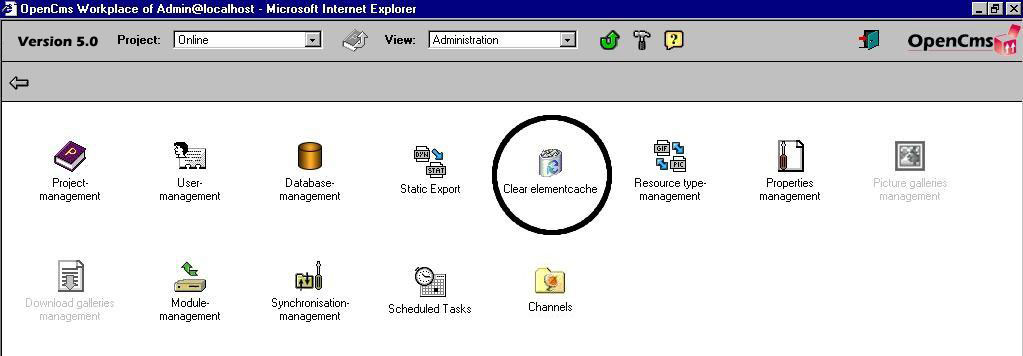
\includegraphics[width=\sgw]
                   {pics/templateMech/clearcache}
\caption[clear elementcache icon]
           {Clear elementcache icon}
           
\label{clear elementcache icon}
\end{center}
\end{figure}

This administration-icon is only visible for administrators 
and only if the element cache has been enabled in the opencms.properties. 
When this point is selected a window will pop up and show the number of uris and elements
that are actually in the cache. You can then select to clear the cache or cancel the 
operation.

\subsubsection{Using the element caching in your own template classes}
The class {\class CmsCacheDirectives} \index{CmsCacheDirectives} provides the opportunity for 
the module developer to specify how pages will be cached with the element cache. 
Every template class has to implement the method {\meth getCacheDirectives()}. Here is
a sourcecode example how this could be done:

\index{getCacheDirectives()}
\begin{java}
public  CmsCacheDirectives getCacheDirectives(CmsObjet cms,\\
\jtabb      String templateFile, String elementName,\\
\jtabb      Hashtable parameters, String templateSelector) \{\\
\jtaba      // create a CmsCacheDirectives object:\\
\jtaba      CmsCacheDirectives cd = \\
\jtabb          new CmsCacheDirectives(true, false, false, false, true);\\
\jtaba      // adding the group to the cache key:\\
\jtaba      cd.setCacheGroups(true);\\
\jtaba      // return the CacheDirectives:\\
\jtaba      return cd;\\
\}\\
\end{java}

(The methods {\meth isCacheable()} \index{isCacheable()} 
and {\meth getKey()} that were used to control the caching for
a pre-eliminary version of the element cache are no longer necessary and will not be supported in future releases.) 
Inside this method an object of type {\class CmsCacheDirectives} is created and returned. 
This object contains information how the element should be cached.
So far the class {\class CmsCacheDirectives} has been used to store informations about server 
and client-side caching and streaming. In addition this class now stores informations 
about the internal caching. These informations specify the different variants of elements 
that will be cached. 

The class {\class CmsCacheDirectives} provides three different constructors:
\begin{itemize}
\item 
\begin{java}
CmsCacheDirectives(boolean internal, boolean proxyPriv,\\
\jtabb      boolean proxyPub, boolean export, boolean stream)\\
\end{java}

This constructor sets the values for:
\begin{itemize}
\item internal: the element can be cached in the element cache
\item proxyPriv: the proxy private flag in the http-response header can be set
\item proxyPub: the proxy public flag in the http-response header can be set
\item export: the element can be exported (static export)
\item stream: the page containing this element can be delivered in streaming mode 
(this means parts of the content can be delivered without waiting until the complete 
content of the page is generated). 
Streaming is usually possible if no redirect is triggered  inside the template class.
\end{itemize}
\item 
\begin{java}
CmsCacheDirectives(boolean)\\
\end{java}
This constructor sets all five boolean parameters of the first constructor to the same boolean value.
\item
\begin{java}
CmsCacheDirectives(boolean internal, boolean stream)\\
\end{java}

This constructor only sets the values for internal caching and streaming. 
The other values can be set seperately to a boolean value by using the methods\\ 
{\meth setProxyPublicCacheable()}, {\meth setProxyPrivateCacheable()} and {\meth setExport()}. 
The values that are not set are determined at runtime by using the following table:


\begin{tabular}{lccc}
& proxy public & proxy private & export \\[0.5ex]
internal cacheable & x & x & x \\
no parameters in the key & & & x \\
user/group not in the key & x & x & x \\
readable for guest-user & x & & x \\
no timeout & & & x \\
no internal flag & x & x & x \\
\end{tabular}

The proxy pub\-lic flag for ex\-am\-ple is set if the in\-ter\-nal cache\-able flag is set, user 
or group
are not in the key, the resource is readable for guest-users and no internal flag is set for 
this resource.
The determination of these values at runtime slows down the caching mechanism, therefore it is
recommended to set these values manually if possible.

\end{itemize}
\subsubsection{Methods in the class CmsCacheDirectives to control the element caching} 
The way elements are cached can be controlled by using several methods of the 
class \\
{\class CmsCacheDirectives}. Essential are the methods that affect the way the cache 
key is generated. If an element is internal cacheable and the caching properties in the\\
{\class CmsCacheDirectives} object have not been adjusted the XML template mechanism generates a variant of this 
element when it is requested for the first time and every following request will 
result in an delivery of this variant from the cache. If someone wants several
variants of an element to be cached he has to specify which variants should be cached. 
For example if an element is different for different groups of users (a login box that 
has a form for guest users to login and a generic message for a user that is already logged 
in) the method {\meth setCacheGroups(true)} provides a way to add the current group of the user to
the cache key. This results in a creation of variants of this element for every different 
group. The complete set of methods to control the caching are:

\begin{itemize}
\item {\meth setCacheUri(boolean uriCache)}\\
If set to true, this method adds the uri to the cache key. 
Variants of the element  for every different uri will be created.

\item {\meth setCacheUser(boolean userCache)}\\
If set to true, this method adds the name of the user to the cache key. 
Variants of the element for every different user will be created. 

\item {\meth setCacheGroups(boolean groupCache)}\\
If set to true, this method adds the name of the group to the cache key.
Variants of the element for every different group will be created.

\item {\meth setCacheGroups(Vector groupNames)}\\
Some elements can be static for specific groups but dynamically for others. 
For example a login box that shows a login form for guest users and a personalized 
message for users that are already logged in. This element can be cached for the 
group Guests but not for the group of users that are logged in. 
For this reason the method {\meth setCacheGroups} is overloaded and provides the 
opportunity to specify a Vector of groupnames  that contains the groups for 
which variants of the element will be cached. For any other groups 
the element will be created dynamically.

\item {\meth setCacheParameters(Vector parameterNames)}\\
The Vector passed to this method contains the name of parameters that should be 
added to the cache key. For every combination of values of these parameters a 
variant of the element will be created.
Another variant will be created if a parameter is not given in the request.

\item {\meth setNoCacheParameters(Vector parameterNames)}\\
This method provides a way to specify the name of parameters that prevent an 
element from beeing cacheable. An registration form for example can be fetched 
from the cache when the form is requested but should be dynamically processed 
when the form is send back. When the name of a parameter that is send with the 
form is passed to this method any occurrence of this parameter in the request will 
cause the element to be created dynamically.

\item {\meth setTimeout(CmsTimeout timeout)}\\
This method provides a way to specify a period of time for which an element is valid. 
The element will be cached but will be created new when this period of time has passed.
This is particulary useful for applications like a news-modul where the news content is
static but should be updated after a certain period of time (e.g. every 60 minutes).
To set a duration of validity a {\class CmsTimeout} object has to be created. So far only one 
constructor which takes a number of minutes exists. The element will then be created new 
at 0:00 am and every x minutes from this point of time.
For example if the timeout was adjusted to 40 minutes the element will be created new at 
0:00 am and then at 0:40 am, 1:20 am, 2:00 am and so forth. The element will at least be 
created new every 24 hours, this means the counting starts new every day at 0:00 am. 
Useful values for the number of minutes are values between 5 and 1440 minutes (24 hours).

A technical note: the element will be checked for validity only when requested. 
An element will therefore be created new when it is requested and the duration of 
validity has passed. When an element is no longer valid all its variants will be deleted 
from the cache. This means the {\meth setTimeout()} method can also be used for elements that 
have several variants. 

\item {\meth renewAfterEveryPublish()}\\
If a project is published every element will be deleted from the cache if the template 
or class of the element has been changed in the project. Also every elements which have variants
for different uris will be deleted from the cache. This is necessary because the hierarchy 
of files and folders in the project could have changed and cause a different output of the
element even if the template of the element hasn't changed. 
Generally the programmer has not to care about deleting elements from the cache. 
In rare cases these rules for deleting elements from the cache may not be sufficient 
(for example if an element itself uses the content of other resources in the virtual file-system).
For this reason the method {\meth renewAfterEveryPublish()} exists to force the system to delete elements
from cache when a project is published.

\subsubsection{Defining caching dependencies with the method registerVariantDeps()}
The method {\meth registerVariantDeps()} allows to define further dependencies for cached elements.
This method can be used inside the {\meth getContent()} method or user-methods to register resources
in the VFS, contentdefinition objects and classes that affect the caching of the current
element. It is not mandatory to use this method when using the element cache, but it allows a more
subtle way to define dependencies and should be used whenever possible.

This is the signature of the method {\meth registerVariantDeps()}:

\begin{java}
protected 
protected void registerVariantDeps(\\
\jtabb     CmsObject cms, String templateName, String elementName,\\
\jtabb     String templateSelector, Hashtable parameters, Vector vfsDeps,\\
\jtabb     Vector cosDeps, Vector cosClassDeps)\\
\jtabb     throws CmsException \\
\end{java}
\end{itemize}

The parameters have the following meaning:

\begin{itemize}
\item[-] cms (type {\class org.opencms.file.CmsObject}) provides access to system resources.
\item[-] templateName (type {\class java.lang.String}) the absolute path to the template. This parameter
is passed to the {\meth getContent()} method and can be get in a user-method  by calling {\meth getAbsoluteFilename()}
on the {\class A\_CmsXmlContent} object.
\item[-] elementName (type {\class java.lang.String}) only needed if this parameter is used in the {\meth getCacheDirectives()}, can be null otherwise.
\item[-] templateSelector (type {\class java.lang.String}) like the elementName this parameter can be null if it is not used inside the
{\meth getCacheDirectives()} method.
\item[-] parameters (type {\class java.util.Hashtable}) hash table with URL-parameters and other parameters added by the system. 
Inside a user-method the {\name userObject} contains this parameters hash table.
\item[-] vfsDeps (type {\class java.util.Vector}) this Vector contains\\
all {\class com.opencms.CmsResource} objects (not the names of the resources !)
which should force the element's variant to be created new if any of these resorces (files and folders) changes.
\item[-] cosDeps (type {\class java.util.Vector}) this Vector contains\\
{\class com.opencms.defaults.A\_CmsContentDefinition} objects
that are used to create the element and affect its output. When one of these resources changes the element's variant will be created new.
\item[-] cosClassDeps (type {\class java.util.Vector}) Here you can add class objects of content definition classes. If one object
of the class changes the element's variant will be created new.
\end{itemize}

Here is a code sample how the method {\meth registerVariantDeps()} is used in the standard navigation class:

\begin{java}
public Object getNavCurrent(CmsObject cms, String tagcontent\\
\jtabc      A\_CmsXmlContent doc, Object userObject)\\
\jtabc      throws CmsException \{\\
\jtaba // current folder\\
\jtaba String currentFolder =\\
\jtabc cms.getRequestContext().currentFolder().getAbsolutePath();\\
\jtaba // register this folder for changes\\
\jtaba Vector vfsDeps = new Vector();\\
\jtaba vfsDeps.add(cms.readFolder(currentFolder));\\
\jtaba registerVariantDeps(cms, doc.getAbsoluteFilename(),\\
\jtabc    null, null, (Hashtable)userObject,\\
\jtabc    vfsDeps, null, null);\\
\}\\
\end{java}